\documentclass[conference]{IEEEtran}
\hyphenation{op-tical net-works semi-conduc-tor IEEEtran}
\usepackage[bottom=2cm,top=3cm,left=3cm,right=2cm]{geometry}
\usepackage{url}
\makeatletter
\def\ps@pprintTitle{%
	\let\@oddhead\@empty
	\let\@evenhead\@empty
	\def\@oddfoot{\reset@font\hfil\thepage\hfil}
	\let\@evenfoot\@oddfoot
}
\makeatother

\usepackage{babelbib}

\usepackage[brazilian]{babel} % Traduz alguns termos para o português
\usepackage[utf8]{inputenc} % Reconhece acentuação
\usepackage{setspace}
\usepackage{graphicx}


\begin{document}

% paper title
\title{Teoria da Decisão\\Projeto Prático Assistido Por Otimização Multiobjetivo e Métodos de Auxílio à Tomada de Decisão}


% author names and affiliations
% use a multiple column layout for up to three different
% affiliations
\author{\IEEEauthorblockN{Rafael Carneiro de Castro}
\IEEEauthorblockA{\\Eng. de Sistemas - UFMG\\
Matrícula: 2013030210\\
Email: rafaelcarneiroget@hotmail.com}
\and
\IEEEauthorblockN{Vinícius Felicíssimo Campos}
\IEEEauthorblockA{\\Eng. de Controle e Automação - UFMG\\
	Matrícula: 2015035235\\
	Email: viniciusfc95@gmail.com}
\and
\IEEEauthorblockN{Davi Pinheiro Viana}
\IEEEauthorblockA{\\Eng. de Sistemas - UFMG\\
	Matrícula: 2013029912\\
	Email: daviviana22@gmail.com}
}

\maketitle

\begin{abstract}
Abordagem de forma conjunta de grande parte dos conceitos vistos na disciplina "ELE088 - Teoria da Decisão", através de um problema relacionado ao gerenciamento ótimo da política de manutenção de um conjunto de equipamentos de uma empresa. O problema foi resolvido através de modelagem e implementação multiobjetivo e, para verificar a resolução do problema, é apresentado um indicador de qualidade. Além disso, foram utilizados alguns métodos de auxílio à tomada de decisão.
\end{abstract}

\IEEEpeerreviewmaketitle

\section{Introdução}
O presente trabalho tem o objetivo de resolver um problema de otimização multiobjetivo e, utilizando técnicas escalares de decisão assistida estudadas em sala de aula, encontrar a melhor solução para este problema, colocando em prática grande parte dos conceitos da matéria.

O problema a ser resolvido é o seguinte: \emph{Deseja-se determinar a política de manutenção ótima para cada um dos 500 equipamentos de	uma empresa, considerando-se a minimização do custo de manutenção e a minimização do custo de falha esperado.}

No problema, o custo de manutenção total é a soma dos custos dos planos de manutenção adotados para todos os equipamentos. Sendo que, o valor do custo de cada plano de manutenção é dado. O custo esperado de falha de cada equipamento $i$, sob o plano de manutenção $j$, é o produto da probabilidade de falha ($p_{i,j}$) e o custo de falha do equipamento (este último é dado). O
custo esperado de falha total é a soma dos custos esperados de falha de todos os equipamentos.

Deve ser feita a formulação e resolução do problema multiobjetivo e o resultado encontrado deve ser avaliado baseado no indicador de qualidade hipervolume (s-metric). Esse indicador é utilizado para mensurar as propriedades de convergência e diversidade da fronteira Pareto "aproximada" obtida.

Além disso, deve ser aplicada também a utilização de técnicas de análise de decisão ELECTRE II, PROMETHEE II \emph{fuzzy} e AHP para decidir qual a melhor solução dentre as encontradas para o problema.

\section{Desenvolvimento}
\subsection{Formulação do Problema:}
A formulação do problema foi dividida em duas partes, como é discutido a seguir:

\subsubsection{Minimização do custo de manutenção total} Em primeiro
momento, é preciso construir uma função objetivo e suas eventuais restrições para minimização do custo de manutenção total. Considerando $C_i(x_i)$ como o custo de manutenção do equipamento $i$ em função do plano de manutenção $x_i$, têm-se a seguinte formulação:

\begin{equation}
\mathrm{min}\ \sum_{i=1,}^{n} C_i (x_i) 
\label{sum_cm}
\end{equation}

sujeito a:
\begin{equation}
x_i \in \mathcal{X}\ \forall i\ \in 1, ..., n
\label{rest1_cm}
\end{equation}
\begin{equation}
C_i \in \mathcal{C}\ \forall i\ \in 1, ..., n
\label{rest2_cm}
\end{equation}
Em que $n$ é o número de equipamentos que, no caso do problema a ser resolvido, é igual a 500. A equação \ref{sum_cm} representa o custo de manutenção total que é o somatório dos custos de manutenção de cada equipamento $i$. A restrição \ref{rest1_cm} indica que cada equipamento $i$ pode ter um plano de manutenção $x_i$ que esteja dentro do conjunto $\mathcal{X}$ de planos pré-definidos, no caso do problema, $\mathcal{X} = \{1,2,3\}$. A restrição \ref{rest2_cm} indica que o custo de manutenção de cada equipamento também deve estar dentro de um conjunto pré-definido $\mathcal{C}$ que depende do plano de manutenção.

\subsubsection{Minimização do custo esperado de falha total}

\subsection{Algoritmo de Solução:}
Nesta seção serão discutidos e exibidos os algoritmos para solução do problema multiobjetivo.

Olhando para a equação \ref{sum_biobj} é possível perceber que, minimizando o custo de cada equipamento, minimiza-se também o somatório dos custos. Assim, para resolução do problema biobjetivo foi utilizada uma estratégia gulosa. Nela, para cada equipamento, é feito um teste com cada um dos planos de manutenção e é escolhido aquele que gera menor custo. Têm-se então, um algoritmo cuja complexidade é O($n\cdot m$) em que $n$ é o número de equipamentos e $m$ é o número de planos de manutenção. No caso do problema a ser resolvido no trabalho, para cada par de pesos escolhido (encontrar solução da fronteira Pareto), são feitas 1500 avaliações da função objetivo. Segue, abaixo, um pseudocódigo do funcionamento do algoritmo:

\begin{algorithm}
	\caption{Estratégia gulosa}
	\begin{algorithmic}[1]
		\For{$i = 1$ to ${n}$}
			\State $cBest = w_1 \cdot c_m(\mathcal{X}_1) + w_2 \cdot c_f(\mathcal{X}_1)$
			\State $x_i = \mathcal{X}_1$
			\For{$j = 2$ to ${m}$}
					\If {$(w_1 \cdot c_m(\mathcal{X}_j) + w_2 \cdot c_f(\mathcal{X}_j)) < cBest$}
					\State $cBest = w_1 \cdot c_m(\mathcal{X}_j) + w_2 \cdot c_f(\mathcal{X}_j)$
					\State $x_i = \mathcal{X}_j$
					\EndIf
			\EndFor
		\EndFor
		
	\end{algorithmic}
\end{algorithm}

Essa estratégia foi escolhida por ser simples de implementar e por retornar uma solução exata para o problema. Além disso, é uma solução relativamente barata computacionalmente e que retorna o resultado rapidamente.

O algoritmo que utiliza a estratégia gulosa para resolver a função objetivo pode ser encontrado no arquivo \texttt{Guloso.m} e o algoritmo que implementa a \emph{Soma Ponderada} variando os pesos da função objetivo pode ser encontrado no arquivo \texttt{SomaPonderada.m}, ambos no mesmo diretório deste relatório.

\subsection{Resultados:}
Os algoritmos foram implementados e, na \emph{Soma Ponderada}, foram encontradas 1000 soluções na fronteira pareto, variando os pesos da seguinte forma: $w_1$ varia de 0 a 1 com o passo igual a $0,001$ e $w_2 = 1 - w_1$. Foi encontrada a seguinte fronteira Pareto:

\begin{figure}[h]
	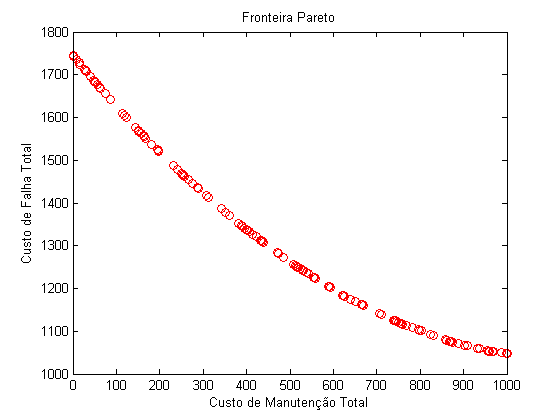
\includegraphics[width=8cm]{img/pareto.png}
	\caption{Froteira Pareto encontrada}
	\label{fig:pareto}
\end{figure}


\subsection{Análise baseada no Hipervolume}
Com o objetivo de avaliar a Fronteira Pareto encontrada, foi utilizada a análise baseada no indicador de qualidade hipervolume (s-metric). Segundo a especificação do trabalho, um bom valor para o HVI (Valor do Hipervolume) deveria estar acima de $0,6$. Utilizando o algoritmo fornecido pelo professor, foi feita uma execução com a Fronteira Pareto encontrada e o valor de HVI foi igual a $0,621246$. Conclui-se, então, que a fronteira encontrada convergiu para uma quantidade boa de soluções e que pode ser utilizada na análise de tomada de decisão da melhor solução.

\section{Tomada de Decisão Assistida}

\section{Conclusão}


\begin{thebibliography}{1}

\bibitem{notas de aula}
Notas de aula do professor Lucas Batista da disciplina \emph{ELE088 Teoria da Decisão}. 2017.

\bibitem{livro}
ARENALES, Marcos et al. Pesquisa operacional: para cursos de engenharia. Rio de Janeiro: Elsevier, 2007

\end{thebibliography}


% that's all folks
\end{document}


